% ex: tw=74 ts=4 sw=4
\documentclass[dvips,10pt,twocolumn]{article}
\usepackage[utf8]{inputenc}
\usepackage[normalem]{ulem}
\usepackage{amsmath}
\usepackage{xkeyval}
\usepackage[bookmarksnumbered,frenchlinks]{hyperref}
\hypersetup{pdfborder=0 0 0}
\usepackage{multirow}
\usepackage{todonotes}
\usepackage[english]{babel}
\usepackage{tabulary}
\usepackage{tabularx}
%\usepackage{fullpage}
%\usepackage{natbib}
\usepackage[all]{hypcap}
\title{802.16-2009 OFDM PHY - Transmitter Portion}
\author{Jonathan Huang \and Cody Schafer \and Luke Steepy}
\date{\today}
\begin{document}
\maketitle

\section{Project Overview}
We are developing a minimal 802.16-2009 OFDM Transmitter PHY.  This PHY
supports only QPSK-1/2 modulation-convolution rate. Additionally, any
components not relevant to unlicensed bands are omitted.  All optional items
are omitted.

This PHY requires the cooperation of a MAC layer implementation which is
compliant with the 802.16-2009 standard in order for the compliance
expectations (\autoref{sec:comply}) to be met.

\begin{figure}
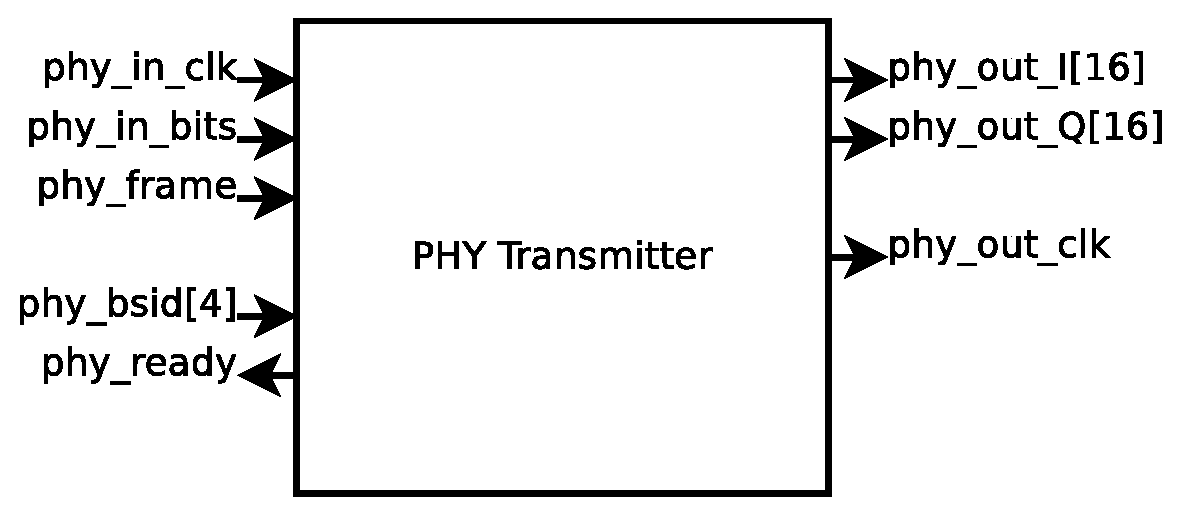
\includegraphics[width=0.5\textwidth]{t_block.eps}
\caption{Overview block diagram of the transmitter}
\end{figure}

\todo[inline]{Derive the product from the needs}

	\subsection{End Market Expectations}
	Currently IEEE 802.16, also known as ``WiMAX'', has seen little
	deployment in the United States and western Europe while being
	moderately deployed in Asian nations and Eastern European markets.
	To be useful in western areas, WiMAX has to effectively compete
	with both consumer owned Wifi hot-spots and the various cell phone
	networks. Given the impressively low cost of both cellular and Wifi
	(802.11) systems combined with the expectation that they work well
	in mobile devices, this physical layer (PHY) targets both
	simplicity (to reduce cost) and reduced power consumption.

	\subsection{Degree of standards compliance and scope limitations}
	\label{sec:comply}
	The 802.16 standard specifies multiple layers of a WiMAX device,
	including a ``Service-specific convergence
	sublayer''~\cite[section 5]{IEEE:802.16}, a MAC
	sublayer~\cite[section 6]{IEEE:802.16}, a Security
	sublayer~\cite[section 7]{IEEE:802.16}, and the Physical
	layer~\cite[section 8]{IEEE:802.16}. 
	
	The PHY, while being described within section 8 of the 802.16-2009
	document, is additionally subject to certain constraints and
	requirements stipulated within the other sections.  These sections
	where only utilized to the extent to which they apply to design of
	the PHY component.

	Applicable sections of \cite{IEEE:802.16}.
	\begin{itemize}
		\item Section 8.3 - OFDM description
		\item Section 8.3.3.4.1 - Data Modulation: implementation
			is not compliant with this section, only QPSK
			modulation is supported.
		\item 8.3.3.4.3 - Rate ID encodings: not compliant with
			this section, only the QPSK-1/2 rate ID is supported.
		\item 8.3.5.1.1 - DL subchannelization: Rate ID
	\end{itemize}

\section{Electrical Characteristics}
All voltages of logic levels are defined by the FPGA on which the product's
code is placed.

\todo[inline]{Need these defined}

\section{OFDM Parameters}

\subsection{Primitive Parameters}

\begin{description}
	\item[BW]: This is the nominal channel bandwidth.
	\item[$N_{used}$]: Number of used subcarriers.
	\item[n]: Sampling factor. This parameter, in conjunction with BW
		and $N_{used}$ determines the subcarrier spacing, and the
		useful symbol time.
	\item[G]: This is the ratio of CP time to ``useful'' time.
\end{description}


\todo[inline]{Insert a table of the values that are fixed by the standard and our
implimentation limitations}

\subsection{Derived Parameters}

\begin{description}
	\item[$N_{FFT}$]: Smallest power of two greater than $N_{used}$
	\item[Sampling Frequency]: $F_s = floor ( n \cdot BW / 8000 )
		\times 8000 $
	\item[Subcarrier spacing]: $\Delta f = F s / N_{FFT} $
	\item[Useful symbol time]: $T_b = 1 / \Delta f$
	\item[CP Time]: $T_g = G \cdot T_b$
	\item[OFDM Symbol Time]: $T_s = T_b + T_g$
	\item[Sampling time]: $T_b / N_{FFT}$
\end{description}

\todo[inline]{Tables of valid values for each of the derived values}

\section{External Interface to the PHY Transmitter}
\label{sec:frame}
The MAC interfaces with the PHY module by sending frames (with the
appropriate headers and padding included) as a stream of bits.  These bits
are clocked via the \textbf{mac\_clk\_in} line, and must only be sent when
the \textbf{mac\_sending\_frame} line is high.  The state of the
\textbf{mac\_sending\_frame} line must be low when not sending a frame, and
must be lowered and raised between frames that would otherwise be abutting.
The frequency of \textbf{mac\_clk\_in} must be less than or equal to half
of the \textbf{phy\_clock}.

The \textbf{phy\_ready} line is a signal to the mac that it is ready for a
new frame to be inputed, and should not be ignored.

The structure of individual frames detailed in section 8.3.5 of IEEE
802.16-2009.  Each frame contains a header, up to 4 DL sub-frames (each with
their own structure also defined in IEEE802.16-2009 section 8.3.5) and some
number of UL sub-frames.  Note that due to fixing certain implementation
parameters, some fields are constrained further than mentioned within the
standard.

\begin{description}
	\item[Frame Header - Rate\_ID] is fixed at '1' indicating QPSK
		modulation with a code rate of $1 over 2$.
	

\end{description}
\todo[inline]{Determine Full inputs and outputs}

\begin{table*} \begin{tabularx}{\textwidth}{c|c|c|X}
	\label{tbl:extern-io}
	Name & Width & Direction & Description\\ \hline

	\texttt{phy\_out\_I} & 16 & O & The real component of the output,
	clocked by \texttt{phy\_out\_clk} \\

	\texttt{phy\_out\_Q} & 16 & O & Imaginary component of the output,
	clocked by \texttt{phy\_out\_clk} \\

	\texttt{phy\_out\_clk} & 1 & O & Clocks out the I and Q values
	produced by the PHY. \\

	\texttt{phy\_in\_bits} & 1 & I & Input bitstream from a MAC
	device. \\

	\texttt{phy\_in\_clk} & 1 & I & Clock at which the input bitstream
	\texttt{phy\_in\_bits} should be sampled. \\

	\texttt{phy\_in\_frame} & 1 & I & Set low while the current set of
	bits is from the same frame. Must be set high for one clock cycle
	between frames. \\

	\texttt{bsid} & 4 & I & The lower four bits of the BSID, a unique
	identifier.
\end{tabularx}
\caption{External Interface to the PHY transmitter.}
\end{table*}

\section{Internal Interfaces}
This section covers the interfaces for internal structures within the PHY
transmitter which are not exposed for use by the MAC or any other interfacing
hardware.

\autoref{tbl:internal-common-wire} shows some of the common signals for
the internal interfaces.

\begin{table*}
\begin{tabulary}{\textwidth}{c|C|L}
	\label{tbl:internal-common-wire}
	Name & Active Level & Meaning \\ \hline
	
	\texttt{*\_valid} & high & Indicate the source outputting the signal
	is also outputting data (clocked via the \texttt{phy\_clock}) which
	should be processed by the next item in the chain. \\

	\texttt{*\_bits} & high & A serial stream of bits clocked by
	\texttt{phy\_clock}. Only valid when the corresponding
	\texttt{*\_valid} line is also active. \\

	\texttt{*\_flag} & high & Set active for a single clock cycle
	before becoming inactive again.
\end{tabulary}
\caption{Common signals used internally}
\end{table*}

Each block of the transmitter connected via direct wiring (without a
buffer) is given the same clock. Each block reads its inputs on alternating
clock edges such that two adjacent units read and write on different edges.
This is done so that outputted data does not change while being read.

%% FRAME

\subsection{Frame Handler}
\begin{description}
	\item[Responsible person] Cody Schafer
	\item[Estimated gates] 2000
	\item[Estimated bitstream delay] 2 clock cycles for a bit to be
		processed 
\end{description}

Is given a bitstream directly from the MAC device, expected to be able to
clock in this bit stream at the rate defined by the MAC. Data and
parsed configuration is sent to the Burst Handler (\autoref{sec:burst})
to be processed and outputed.

Inputs and outputs are listed in \autoref{tbl:frame-io}.

\begin{table*} \begin{tabularx}{\textwidth}{c|c|c|X} \label{tbl:frame-io}
	Name & Width & Direction & Description \\ \hline

	\texttt{frame\_in\_bits} & 1 & I & Input bitstream, clocked via
	\texttt{frame\_in\_clk}. \\

	\texttt{frame\_in\_clk} & 1 & I & Positive edge indicates that data on
	\texttt{frame\_in\_bits} should be read. \\
	
	\texttt{frame\_in\_valid} & 1 & I & Set high while the current series
	of bits is part of the same frame. \\

	\texttt{burst\_reset} & 1 & O & reset line to the burst handler
	(\autoref{sec:burst}). \\

	\texttt{burst\_bits} & 1 & O & Bits to the burst handler. \\

	\texttt{burst\_valid} & 1 & O & indicates the bitstream
	\texttt{burst\_bits} is valid and should be processed. \\


	\texttt{frame\_num} & 4 & O & The frame number parsed from the header
	structures. \\

	\texttt{iuc} & 4 & O & The UIUC or DIUC field, parsed from the header
	stuctures. Only valid for the currently outputed frame. \\

	Something about subchannels & ? & O & Indicates something about
	subchannels to things. Need documentation as to what the other logic
	blocks require before this can be pinned down. \\

\end{tabularx} \caption{Frame Handler interface description} \end{table*}

%% BURST

\subsection{Burst Handler} \label{sec:burst}
\begin{description}
	\item[Responsible person] Cody Schafer 
	\item[Estimated gates] 2000 
	\item[Estimated data bitstream delay] 2 clock cycles for a bit to be
		processed, could be cut to zero by bypassing.
\end{description}

Bursts are composed of multiple OFDM symbols. OFDM symbols are composed of
multiple sub-channels(??). 

\autoref{tbl:burst-io} shows the burst interface inputs and outputs.
Across a single burst initialization of the pipeline hardware will not
change.

\begin{table*} \begin{tabularx}{\textwidth}{c|c|c|X}
	\label{tbl:burst-io}
	Name & Width & Direction & Description \\ \hline
	
	\texttt{burst\_reset} & 1 & I & Imediately resets the burst handler.
	\\

	\texttt{iuc} & 4 & I & The UIUC or DIUC field (depending on uplink
	or downlink state). Used by randomizer. \\
	
	\texttt{bsid} & 4 & I & Used by randomizer. \\
	
	\texttt{frame\_num} & 4 & I & Used by randomizer. \\

	\texttt{burst\_in\_bits} & 1 & I & Input bitstream. \\

	\texttt{burst\_in\_valid} & 1 &  I & Indicates the input bitstream
	\texttt{burst\_in\_bits} is valid. \\

	\texttt{rand\_iv} & 15 & O & The initialization for
	the randomizer's internal register. \\

	\texttt{rand\_reload} & 1 & O & Instructs the randomizer to reload
	it's internal register with a new one outputed on
	\texttt{rand\_iv}. \\

	\texttt{burst\_out\_bits} & 1 & O & Output bitstream. Sent to the
	randomizer for first portion of processing. \\

	\texttt{burst\_out\_valid} & 1 & O & Indicates output is valid.
	Also attached to the randomizer. \\

	\texttt{subchan\_data} & ? & I & See \autoref{tbl:frame-io}. This
	should be decoded to the useful items or simply passed along the
	pipeline.

\end{tabularx}
\caption{Interface definition for the Burst Handler.}
\end{table*}

%% RAND

\subsection{Randomizer}
\label{sec:rand}
\begin{description}
	\item[Responsible person] Cody Schafer 
	\item[Estimated gates] 1000
	\item[Estimated data bitstream delay] 8 clock cycles for a bit to be
		processed, could be cut to zero by bypassing.
\end{description}

The randomizer operates as a shift register with an initial value
determined by the PDU (packet data unit, one half of a frame) header
and whether it is a UL (uplink) or DL (downlink) PDU.

\autoref{tbl:rand-io} describes the inputs and outputs of the
randomizer.

\begin{table*} \begin{tabularx}{\textwidth}{c|c|c|X}
	\label{tbl:rand-io}
	Name & Width & Direction & Description \\ \hline

	\texttt{rand\_in\_bits}  & 1  & I & Uncoded input bitstream to the
	randomizer (this is the first step in the encoding process).\\

	\texttt{rand\_in\_valid} & 1  & I & Indicates the input bitstream

	\texttt{rand\_in\_bits} is valid and should be read. \\

	\texttt{rand\_out\_bits} & 1  & O & Output bitstream. \\
	
	\texttt{rand\_out\_bits} & 1  & O & Indicates the output bitstream
	is valid. \\

	\texttt{rand\_iv}        & 15 & I & Initialization data for the
	internal register. \\

	\texttt{rand\_reload}    & 1  & I & Indicates the internal
	register should be loaded with \texttt{rand\_iv}. \\

	\texttt{rand\_reset}     & 1  & I & Resets all internal state
	imediately. The internal register is loaded from
	\texttt{rand\_iv}.

\end{tabularx}
\caption{Randomizer interface definition.}
\end{table*}
	
%% FEC

\subsection{Forward Error Correction}
	\label{sec:fec}
	This is a Reed-Solomon and convolution coding combination
	which is applied per frame. Within the standard, different
	RS (Reed-Solomon) codes and CC (convolution code) rates are
	used for varying modulation types. As we have fixed the
	modulation and code rate to QPSK-1/2, one two of the RS
	code and CC rate pairs are needed, as indicated in the
	\autoref{tbl:fec-param}.

	See \autoref{tbl:fec-io} for a listing of the inputs and outputs.
	
	\begin{table*}
		\begin{tabularx}{\textwidth}{X|X|X|X|X|X}
		\label{tbl:fec-param}
			Modulation & Uncoded block size (bytes) &
			Coded block size (bytes) & Overall coding
			rate & RS code & CC code rate \\ \hline
			QPSK & 24 & 48 & 1/2 & (32,24,4) & 2/3 \\
		\end{tabularx}
		\caption{Forward Error correction rates}
	\end{table*}

	\begin{table*} \begin{tabularx}{\textwidth}{c|c|c|X}
		\label{tbl:fec-io}
		Name & Width & Direction & Description \\ \hline

		\texttt{fec\_in\_bits} & 1 & I & Input bitstream, processsed by randomizer.
		\\

		\texttt{fec\_in\_valid} & 1 & I & Indicates the input bitstream
		\texttt{fec\_in\_bits} should be read.\\

		\texttt{fec\_out\_bits} & 1 & O & Output bitstream, has FEC
		applied. Will be longer than input bitstream. \\

		\texttt{fec\_out\_valid} & 1 & O & Indicates the output bitstream
		is valid (the data on it should be read and processed) \\

		\texttt{rate\_id} & 4 & I & The type of modulation used. See
		\autoref{tbl:rate-id} for possible values.

	\end{tabularx} \caption{FEC interface description} \end{table*}

	Estimated Gates: 2k \\
	Responsible Person: Luke.

	\subsection{FEC to Interleaving Circular buffer}
	\label{sec:fec_buffer}

	\begin{description}
		\item{Inputs:} \begin{description}
			\item[bits\_from\_fec]
			\item[en\_from\_fec], indicates the incoming
				bit-stream is valid
			\item[fec\_buf\_adv\_flag] set high for a
				single clock cycle by the consumer to
				indicate it has consumed the
				presently outputted data block.
		\end{description}
		\item{Outputs:} \begin{description}
			\item[fec\_buffer\_flag], 
			\item[fec\_buffer\_out{[96]}], set high to indicate
				output bit-stream is valid.
		\end{description}
	\end{description}

	Takes \textbf{bits\_from\_fec} (triggered via
	\textbf{en\_from\_fec}) and places them in a circular
	buffer. When the number of buffered bits equals the block
	size of the Interleaver (set at 96 bytes or 768 bits), the
	\textbf{fec\_buffer\_done} flag is set. Data is outputted
	via \textbf{fec\_buffer\_out[96]}

	Estimated Gates: 1K \\
	Responsible Person: Cody

	\subsection{Interleaving}
	\label{sec:interleaving}
	
	All encoded data bits will be interleaved by this block interleaver. The
	block size is defined by the number of coded bits per allocated subchannels 
	per OFDM symbol ($N_{cbps}$). 
 
	 \begin{center}
  	\begin{tabular}{|c|c|c|c|c|c|}
	\hline
	\multicolumn{6}{|c|}{Block sizes of the Interleaver} \\ \hline
	\multicolumn{6}{|c|}{$N_{cbps}$} \\ \hline
  	& 16 subchannels & 8 & 4 & 2 & 1 \\ \hline
	QPSK & 384 & 192 & 96 & 48 & 24 \\ \hline
	\end{tabular}
  	\end{center}

	Interleaving is a two step type operation. The first step ensures adjacent 
	coded bits are mapped onto nonadjacent subcarriers and the second step 
	ensures bits are mapped alternately onto less and more significant bits of
	the constellation. The second step is done to avoid long runs of lowly
	reliable bits.
	 
	The permutations are dependent on the number of coded bits per subcarrier
	($N_{cpc}$), which is defined by the type of modulation and the index of the
	coded bit before permutation (k).

	For our implementation, as we are only using QPSK modulation,
	$N_{cpc} = 2$.
	
	k : index of coded bit before first permutation

	$m_{k}$ : index after first permutation

	$j_{k}$ : index after second permutation 

  First permutation equation :
  \begin{equation}
  m_k = (N_{cbps}/12)*k_{mod12}+floor(k/12)
  \end{equation}

	Second permutation equation :
	\begin{equation}
	s=ceil(N_{cpc}/2) \\
	\end{equation}
	\begin{eqnarray}
	j_k = s*floor(m_{k}/s)+(m_{k}+N_{cbps}- \nonumber \\
		floor(12*m_k/N_{cbps}))_{mod(s)}
	\end{eqnarray}

	After the interleaving the first bit out of the interleaver would map to the
	MSB for the constellation mapping. 
	
	\begin{table*}
		\begin{tabularx}{\textwidth}{X|X|X|}
		\label{tbl:interleave}
			Signal name & From/To &
			Description \\ \hline
			fec\_buffer\_out & From Buffer & A block of $N_{cbps}$ bits are read
			along this line \\ \hline
			fec\_buffer\_done & From Buffer & Indicates on high that a block of
		 	encoded bits are ready to be read \\ \hline
			interleave\_reset & From Control Logic & On high, causes reset\\ \hline
			interleave\_out\_enable & To Constellation Mapping & On high output
			line of bits is valid and ready to read \\ \hline
			interleaved\_bits & To Constellation Mapping & Interleaved bits are
			sent on this line \\ \hline
		\end{tabularx}
		\caption{Interleaver IO signals}
	\end{table*}
	
  \subsubsection{Testing and Verification}
  
  The Interleaver operation can be verified by inputting a known block of bits
  and observing the output. With the equations defined in the IEEE 802.16
  document, the appropriate Interleaver output can be calculated and compared
  directly. 
  
  *Add example test inputs and outputs. 

  Estimated Gates: 2K
  Responsible Person: John

	\subsection{Constellation Mapping}
	\label{sec:constellation}

	Input is bit stream, output is (I,Q).
	
	Estimated Gates: 4K \\
	Responsible Person: Luke

	\subsection{Pilot Sub-carrier Insertion}
	\label{sec:pilot}

	Input is (I,Q) pair, output is (I,Q) pair with pilot subcarriers
	inserted at some points (fixed).

	Estimated Gates: 1K \\
	Responsible Person: Luke

	\subsection{Sub-carrier to IFFT Buffer}
	\label{sec:ifft-buffer}
	Insertion into this buffer is ordered but will have random
	jumps around different UL \& DL bursts.

	Block Size = blk\_siz = 200 (the total number of used
	subcarriers)
	
	Buffers blk\_size items each of which has width 2 bits.
	QPSK utilizes both I and Q, amplitude and phase, each with
	a granularity of 2. This means that each item (a pair of I
	\& Q) has 4 possible values and thus 2 bits are needed for
	each.

	Estimated Gates: 2k \\
	Responsible Person: Cody.

	\subsection{IFFT}
	\label{sec:ifft}
	*
	The IFFT 
	IFFT Size: 256 items (each being a complex number)
	\begin{description}
		\item{Inputs:}
		\begin{description}
			\item[ifft\_buf\_has\_block] The count of the last
				block present in the Sub to IFFT buffer
				(\autoref{sec:ifft-buffer})
			
			\item[ifft\_buf\_data{[200][2][??ndepth]}] access
				to the data at the present 'tail' location
				in the buffer
		\end{description}
		
		\item{Outputs:}
		\begin{description}
			\item[ifft\_data\_ready] high when the IFFT has
				processed data.
		\end{description}
	\end{description}

	Estimated Gates: 10k.
	Responsible Person: John.

	\subsection{Cyclic Prefix}
	\label{sec:cyclic_prefix}
	
	The Cyclic Prefix appends to the front of the symbol a copy of the last
 	$256/CP_{rate}$ ($N_{IFFT}/CP_{rate}$) bits. OFDM PHY should allow for four
	(4) rates as defined by 2 bits in the PHY Mode ID field. 

	%\begin{tabular}
	$CP_{rate}$ 1/4,1/8,1/16,1/32
	%\end{tabular} 
	
	
	
	\begin{table}
	\begin{tabulary}{0.5\textwidth}{C|C}
		\label{tbl:param-g-vals}
		Value of \texttt{param\_G} & Ratio of CP time to
		``useful'' time. \\ \hline

		0b00 & 1/4 \\
		0b01 & 1/8 \\
		0b10 & 1/16 \\
		0b11 & 1/32 \\

	\end{tabulary}
	\caption{Values of OFDM parameter G as presented on
	\texttt{param\_G}}
	\end{table}

	\begin{table*}
	\begin{tabularx}{\textwidth}{c|c|c|X}
		\label{tbl:cp-io}
		Name & Direction & Width & Description \\ \hline

		\texttt{param\_G} & I & 2 & The meanings of valid values
		are listed in \autoref{tbl:param-g-vals}. Indicates the
		fraction of CP time to ``useful'' time.
		\\

		\texttt{cp\_in\_bits} & I & 1 & Input bitstream. \\
		
		\texttt{cp\_in\_valid} & I & 1 & Indicates the input
		bitstream \texttt{cp\_in\_bits} is valid. \\

		\texttt{cp\_out\_bits} & O & 1 & Output bitstream. \\

		\texttt{cp\_out\_valid} & O & 1 & Indicates the output
		bitstream \texttt{cp\_out\_bits} is valid. \\

	\end{tabularx}
	\caption{Cyclic Prefix Inputs and Outputs}
	\end{table*}

	\autoref{tbl:cp-io} lists the inputs and outputs to the cyclic
	prefix unit.

	Appends the last Tg items of the previous frame to the start of the
	present frame.  Reads 256 2 bit items from the IFFT, appending Tg
	items to the start of it. It also stores the last Tg items so that
	they may be appended to the next frame from the IFFT.

	Size is fixed at ??

	Estimated Gates: 2k.

	Responsible Person: Cody.

	\subsection{Control Logic}
	\label{sec:ctrl}

\section{Testing Considerations}
\section{Economic Analysis}
\section{Power Consumption}
\section{FPGA Implementation}
  \subsection{Sampling and Clock Rate}
    From the IEEE 802.16 standards document, the sampling rate for
    256-OFDM is defined as
    \begin{equation}
    F_s = BW * 7/6
    \end{equation}
  
  \begin{center}
  \begin{tabular}{c|c}
  Channel Bandwidth & Sampling Rate \\ \hline
  14 MHz & 16.333 MHz \\
  7 MHz & 8.166 MHz \\
  3.5 MHz & 4.083 MHz \\
  1.75 MHz & 2.042 MHz
  \end{tabular}
  \end{center}
  
  This design should be able to run on both the Spartan-3 FPGA and Virtex 4 LX60
  FPGA as they both supply a 500 MHz clock.
  
  \subsection{Power Calculation}
  
  Calculate power based on required clock frequency for the device as well as the
  FPGA specifications for voltage inputs.
  
  Absolute Maximum rating for $V_{in}$ : 4.4 V
  
  Clock frequency required for a 3.5 MHz channel bandwidth : 4.083 MHz
  
  Input capacitance over recommended operating conditions : 10 pF
  \begin{center}
  \begin{equation}
  P = C * V^2 * f = 10 pF * (4.4 V)^2 * 4.083 MHz = 0.18 mW
  \end{equation}
  \end{center}
  \todo[inline]{Is this correct?}
  
	%\subsection{Pin outs}
	%XC3S200-FT256
	%//Top and Bottom View Package FT256 -   %http://www.xilinx.com/support/documentation/package_specs/ft256.pdf 
	%\section{Datasheet(Spartan-3 FPGA}
	%\subsection{Electrical Characteristics}
	%\begin{tabular}
	%\end{tabular}

\bibliography{doc}{}
\bibliographystyle{ieeetr}
\end{document}
